\documentclass{article}
\usepackage{gvv}
\usepackage{gvv-book-bkup}
\begin{document}
\title{GATE Question}
\begin{center}
\begin{tabular}{|m{1cm}|m{13cm}|}
	\hline
	Q.21 & The output of a 2-input multiplexer is connected back to one of its inputs as shown in the figure.
	\begin{center}
		\newline 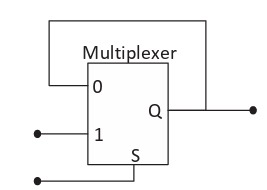
\includegraphics[width=0.3\textwidth,height=30mm]{/storage/self/primary/Assignments/IMG-20231017-WA0029.png}
	\end{center}
		\newline Match the functional equivalence of this circuit to one of the following option. \\
	\hline
	(A) & D Flip-Flop \\
	\hline
	(B) & D Latch \\
	\hline
	(C) & Half-adder\\
	\hline
	(D) & Demultiplexer \\
	\hline
\end{tabular}
\end{center}
\end{document}


